\documentclass[a4paper, 12pt]{article}
\usepackage[a4paper,top=1.5cm, bottom=1.5cm, left=1cm, right=1cm]{geometry}
\usepackage[utf8]{inputenc}
\usepackage{mathtext}
\usepackage{amsmath}
\usepackage{amsfonts}
\usepackage[english, russian]{babel}
\usepackage{indentfirst}
\usepackage{longtable}
\usepackage{graphicx}
\graphicspath{{pictures/}}
\DeclareGraphicsExtensions{.pdf,.png,.jpg}
\usepackage{natbib}
\usepackage{hyperref}
\usepackage{emoji}
\babelfont{rm}{Droid Serif}
\babelfont{sf}{Droid Sans}
\renewcommand{\baselinestretch}{1.3}


\title{Лабораторная работа 1.1.6. Изучение электронного осциллографа}
\author{Платонов Егор}
\date{\today}



\begin{document}
	
\maketitle

\section{Аннотация}

\textbf{Цель работы:} ознакомление с устройством и работой осциллографа, изучение его основных характеристик

\textbf{В работе используются:} осциллограф, генераторы электрических сигналов, соединительные кабели.

\section{Теоретические сведения}
\subsection{Принцип работы осциллографа}
\begin{figure}[h]
    \centering
    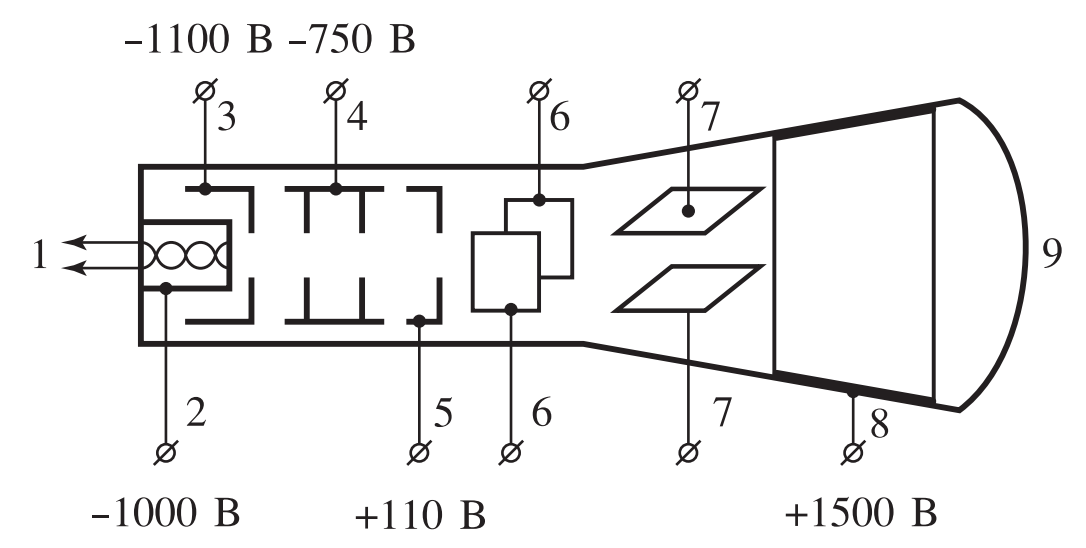
\includegraphics[scale=0.7]{oscilloscope.png}
    \caption{Электронно-лучевая трубка}
    \label{fig:oscilloscope}
\end{figure}

Электронно-лучевая трубка. Основной частью электронного осциллографа, определяющей его важнейшие технические характеристики, является электронно-лучевая трубка (ЭЛТ). Трубка представляет собой стеклянную откачанную до высокого вакуума колбу, в которой расположены (рис. \ref{fig:oscilloscope}): подогреватель катода 1, катод 2, модулятор 3 (электрод, управляющий яркостью изображения), фокусирующий анод 4, ускоряющий анод 5, горизонтально и вертикально отклоняющие пластины 6 и 7, ускоряющий анод 8, экран 9.
Экраном осциллографа является покрытая флюоресцирующим веществом стенка трубки, на которую и попадает электронный пучок.
Электронный пучок формируется системой электродов, называемой
«электронной пушкой»: катод с нагревателем, модулятор, фокусирующий и ускоряющий аноды. С помощью ручек регулировки яркости и фокуса можно изменять потенциалы фокусирующих и ускоряющих
анадов, регулируя таким образом размер, чёткость и яркость пятна на
экране.

Траектория пучка электронов меняется вертикальной и горизонтальной парами отклоняющих пластин (рис. \ref{fig:plates}).
\begin{figure}[h]
    \centering
    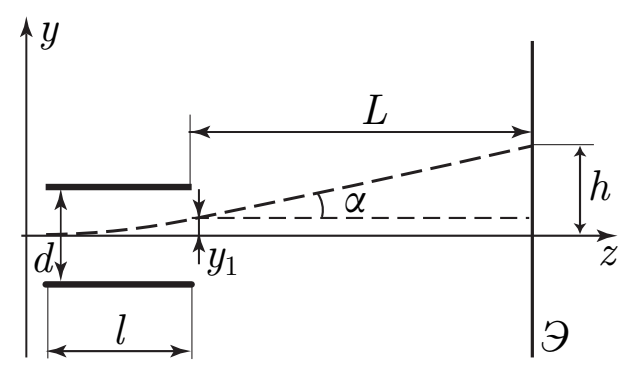
\includegraphics{plates.png}
    \caption{Отклонение луча в электрическом поле пластин}
    \label{fig:plates}
\end{figure}
Описание траектории движения пучка:
\begin{equation}
    z = v_0t
\end{equation}
\begin{equation}
    y=\frac{at^2}{2}
\end{equation}
\begin{equation}
    a=\frac{eE_y}{m}
\end{equation}
Из (1), (2), (3) получаем зависимость координаты $y$ от $z$ (парабола):
\begin{equation}
    y = \frac{eE_y}{2mv_0^2}z^2
\end{equation}
Из (4) получаем угол и смещение при вылете из поля пластины:
\begin{equation}
    y_1 = \frac{eE_y}{2mv_0^2}l^2
\end{equation}
\begin{equation}
    \tg\alpha = \frac{eE_y}{mv_0^2}l
\end{equation}
Из (5), (6) получаем полное смещение:
\begin{equation}
    h = y_1 + L\tg\alpha=\frac{el(l/2+L)}{mv_0^2}E_y = \frac{el(l/2+L)U_d}{dmv_0^2}
\end{equation}
Скорость можно выразить через ускоряющее напряжение на ускоряющем аноде:
\begin{equation}
    \frac{mv_0^2}{2}=eU_a
\end{equation}
Из (7), (8) получаем:
\begin{equation}
    h=\frac{l(l/2 +L)}{2dU_a}U_y
\end{equation}
Найдем чувствительность трубки к напряжению ($K_y$):
\begin{equation}
    K_y=\frac{U_y}{h} = \frac{2dU_a}{l(l/2+L)}
\end{equation}
Аналогично вычисляется чувствительность трубки к напряжению на
второй паре пластин ($K_x$).
\subsection{Развёртка сигнала}
Для получения на экране «изображения»
некоторого электрического сигнала $U(t)$ сам сигнал нужно подать на
вертикальные пластины, на горизонтальные пластины нужно подать напряжение развертки:
\begin{equation}
    U_y(t)=U_{0y}+K_yU(t)
\end{equation}
\begin{equation}
    U_x(t)=U_{0x}+kt,
\end{equation}
где

$U_{0y}$ и $U_{0x}$ - постоянные, задающие смещение графика сигнала

$K_y$ -- коэффициент усиления сигнала по вертикальной оси

$k$ -- постоянная, зависящая от характеристик генератора развертки

\begin{figure}[h]
    \centering
    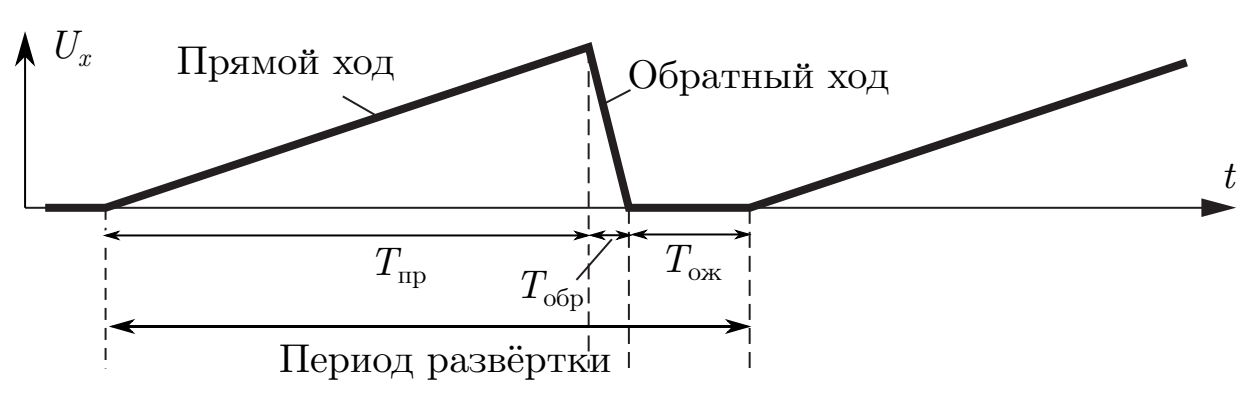
\includegraphics[scale=0.7]{ux.png}
    \caption{Напряжение развертки}
    \label{fig:ux}
\end{figure}

После того, как луч в процессе развёртки дойдёт до края экрана,
развёртка должна быть запущена заново. В результате напряжение
на горизонтальных пластинах будет иметь пилообразную форму. Это напряжение, изображённое на рис. 3, вырабатывает генератор внутренней развёртки осциллографа. В течение времени прямого хода луча напряжение изменяется до максимального значения так, что луч с постоянной скоростью проходит весь экран слева направо. После завершения прямого хода луча начинается процесс обратного хода, когда напряжение развёртки возвращается к первоначальному уровню, а луч переходит в исходное положение в левый край экрана (заметим, что при обратном ходе луча напряжение на модуляторе «запирает» трубку, поэтому свечение экрана не возникает). Скорость изменения напряжения прямого хода развёртки, т. е. масштаб по оси X, задаётся специальной ручкой регулировки, устанавливающей соотношение между временем и числом делений экрана («ВРЕМЯ/ДЕЛ» или «TIME/DIV»). После возврата луч может
стартовать не сразу, а находиться в покое в течение времени ожидания, что позволяет синхронизировать отрисовку сигнала.

\subsection{Синхронизация}
При наблюдении периодических и, особенно, быстропротекающих процессов важно получить на экране осциллографа неподвижное изображение сигнала. Для этого необходимо, чтобы
период развёртки был кратен периоду изучаемого периодического сигнала -- тогда повторная «прорисовка» пройдёт по тому же пути, что и предыдущая.

\begin{figure}[h]
    \centering
    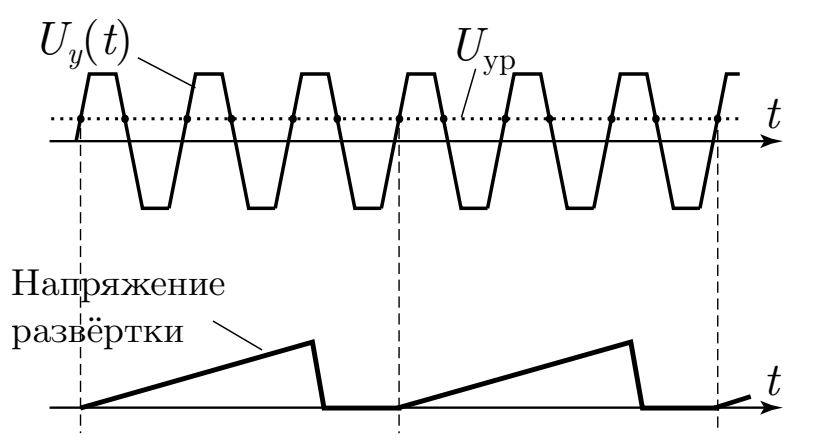
\includegraphics{uyux.png}
    \caption{Синхронизация развёртки по заданному уровню (по нарастанию)}
    \label{fig:uyux}
\end{figure}

Наиболее часто используется способ синхронизации развёртки по
уровню сигнала. Он поясняется осциллограммами на рис. 4. Периодический сигнал произвольной формы $U_y$ сравнивается с некоторым пороговым напряжением $U_ур$ -- уровнем синхронизации (устанавливается ручкой «УРОВЕНЬ» или «LEVEL» блока управления синхронизацией). После попадания в режим ожидания, прямая развёртка не запускается до тех пор, пока величина сигнала $U_y$ не достигнет порогового значения $U_ур$, то есть пока не произойдёт пересечение уровня (сверху вниз или снизу вверх, в зависимости от настроек). Таким образом, регулировка уровня синхронизации позволяет выбрать фазу сигнала в начале развёртки.

\subsection{Фигуры Лиссажу}
Помимо наблюдения развёртки сигналов, в любом осциллографе предусмотрен режим совместной подачи двух сигналов $U_y(t)$ и $U_x(t)$ на вертикальные и горизонтальные отклоняющие пластины. В результате на экране будет наблюдаться результат сложения двух взаимно перпендикулярных колебаний.

Если сигналы:
\begin{equation}
    U_y(t)=U_{0y}\sin(2\pi\nu_y(t)+\phi_y)
\end{equation}

\begin{equation}
    U_x(t)=U_{0x}\sin(2\pi\nu_x(t)+\phi_x)
\end{equation}

являются периодическими с совпадающими или кратными частотами, на экране возникают неподвижные замкнутые кривые, называемые ф и г у рами Лиссажу. Вид фигуры Лиссажу зависит от соотношений между периодами (частотами), фазами и амплитудами складываемых колебаний. Некоторые частные случаи фигур Лиссажу для
разных периодов и фаз показаны на рис. 5.

\begin{figure}[h]
    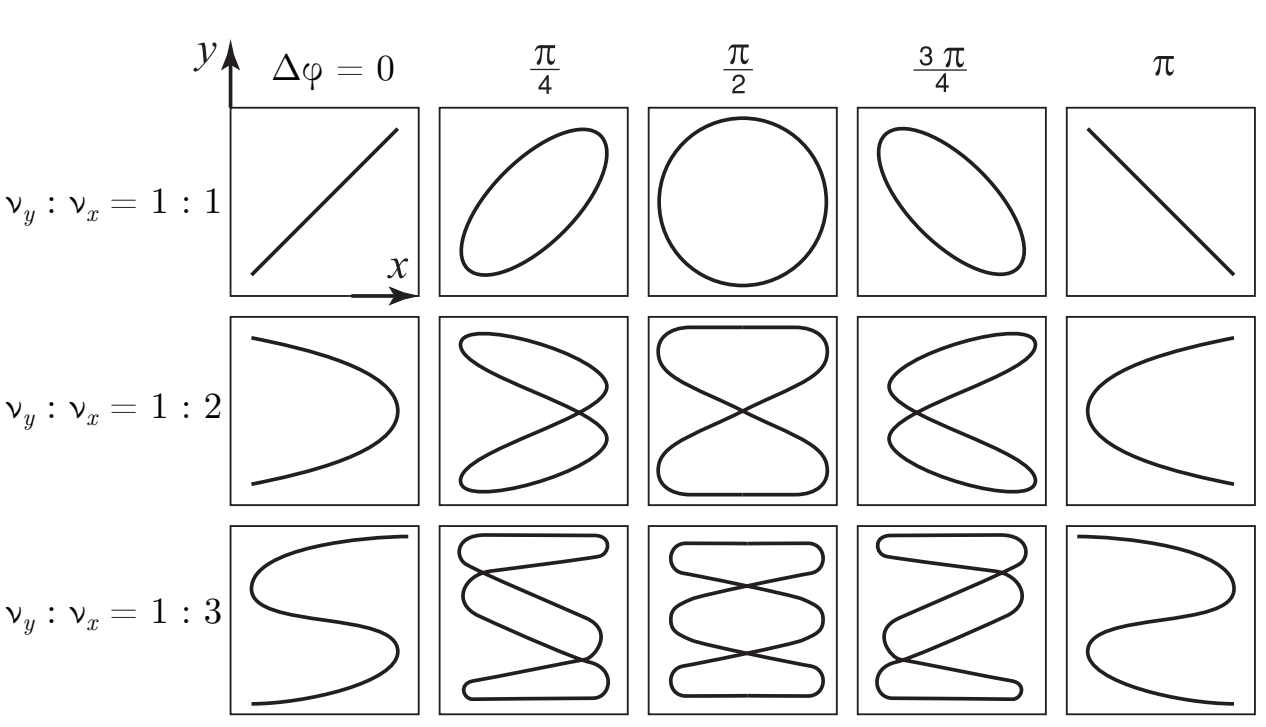
\includegraphics[scale=0.7]{lissajous.png}
    \caption{Фигуры Лиссажу (для колебаний одинаковой амплитуды)}
    \label{fig:lissajous}
\end{figure}

\section{Результаты измерений и обработка данных}

\section{Выводы}

\end{document}